
% --- SLIDE 4: DRIFT PATTERNS ---
\begin{frame}{Drift Comes in Shapes}

    \centering
    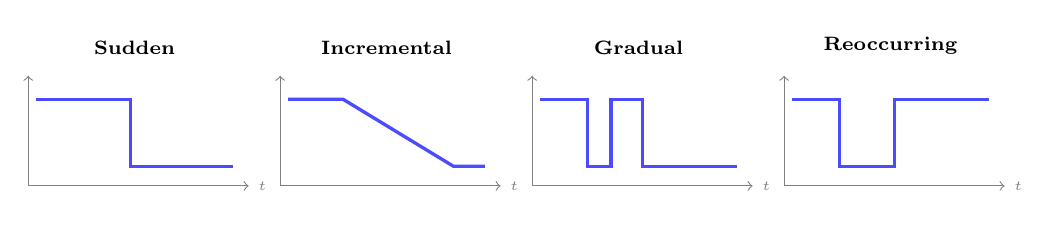
\begin{tikzpicture}[font=\tiny]
        \foreach \lbl/\dx in {{Sudden}/0, {Incremental}/3.2, {Gradual}/6.4, {Reoccurring}/9.6} {
            \begin{scope}[shift={(\dx,0)}]
                \node[font=\scriptsize\bfseries, anchor=south] at (1.35,1.55) {\lbl};
                \draw[->, gray] (0,0) -- (2.8,0) node[right, font=\tiny] {$t$};
                \draw[->, gray] (0,0) -- (0,1.4);
            \end{scope}
        }
        % sudden
        \draw[blue!70, very thick] (0.1,1.1) -- (1.3,1.1) -- (1.3,0.25) -- (2.6,0.25);
        % incremental
        \draw[blue!70, very thick] (3.3,1.1) -- (4.0,1.1) -- (5.4,0.25) -- (5.8,0.25);
        % gradual (oscillates between old and new before settling)
        \draw[blue!70, very thick] (6.5,1.1) -- (7.1,1.1) -- (7.1,0.25) -- (7.4,0.25)
            -- (7.4,1.1) -- (7.8,1.1) -- (7.8,0.25) -- (9.0,0.25);
        % recurring (seasonal)
        \draw[blue!70, very thick] (9.7,1.1) -- (10.3,1.1) -- (10.3,0.25) -- (11.0,0.25)
            -- (11.0,1.1) -- (12.2,1.1);
    \end{tikzpicture}

    \vspace{0.8em}
    \begin{itemize}
        \small
        \item \textbf{Sudden} --- a policy change, a competitor's launch, a pipeline rewrite. Easy to detect,
              hard to prevent.
        \item \textbf{Incremental / gradual} --- the dangerous ones. Any single week looks fine; the year does
              not. Detected only by comparing against a \emph{fixed} reference window.
        \item \textbf{Reoccurring} --- seasonality. \textbf{Do not retrain on this.} Give the model the
              calendar as a feature instead, or you will chase your own tail every December.
        \item A single anomalous window is an \textbf{outlier}, not drift. Do not retrain on one bad Tuesday.
    \end{itemize}

    \vspace{0.4em}
    {\scriptsize Taxonomy after Gama, Zliobaite, Bifet, Pechenizkiy \& Bouchachia,
    ``A Survey on Concept Drift Adaptation,'' \textit{ACM Computing Surveys} 46(4), Article~44, 2014,
    \href{https://dl.acm.org/doi/10.1145/2523813}{DOI:10.1145/2523813}, Figure~2.}

\end{frame}
